% 2016 공주대 워크숍
% 텍 매크로 작성법

\documentclass{beamer}

\usetheme{metropolis}
\metroset{inner/sectionpage=none}
\metroset{outer/progressbar=head}
\metroset{color/block=fill}

\usepackage{kotex}

\hypersetup{pdfencoding=auto}


% title
\title{텍 매크로 작성법}
\subtitle{텍 매크로 작성의 기초와 응용}
\author{남수진}
\date{2016년 11월 5일(토)}
\institute{
  2016 공주대학교 문서작성 워크숍 2016\\
  공주대학교 인문사회과학관 1층 컴퓨터실 107호}


%%
\begin{document}

\maketitle


%
\begin{frame}{매크로 관련 명령어}
  \vspace{4mm}
  \hbox to\hsize{\hss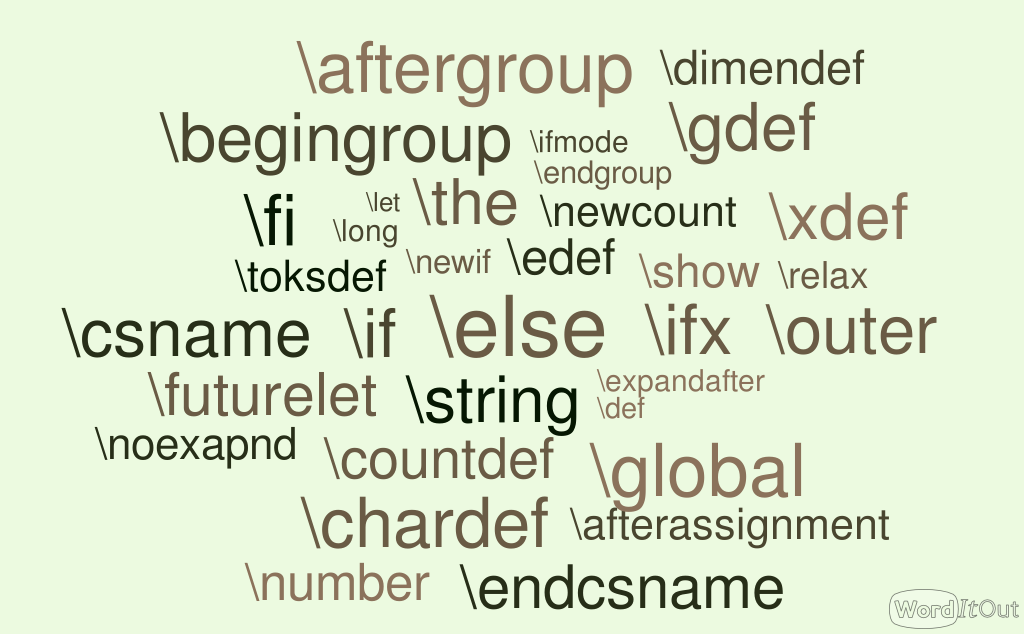
\includegraphics[height=7.5cm]{cs.png}\hss}
\end{frame}


%
\begin{frame}[fragile]{텍의 처리 과정}
  \begin{description}
  \item [입력(input processor)] 파일을 입력받아서 \alert{토큰 리스트}를 만든다.
  \item [전개(expansion processor)] 입력 과정의 결과물인 토큰 리스트를 입력으로 받어서
    새로운 토큰 리스트를 만든다.
  \item [실행(execution processor)]
  \item [출력(visual processor)]
  \end{description}

  \begin{alertblock}{토큰 리스트}
  \verb+{\hskip 36 pt}+\par
  \smallskip
  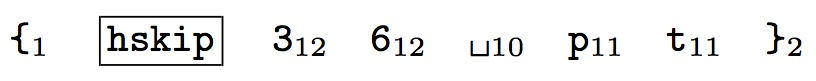
\includegraphics[width=10cm]{tokens.jpg}
  \end{alertblock}
\end{frame}


%
\begin{frame}[fragile]{매크로 정의}
  
  \begin{center}
    \hbox to\hsize{\hss
    \verb+\def+<control sequence><parameter text>%
    \verb+{+<replacement text>\verb+}+\hss}
  \end{center}

  \begin{itemize}
  \item 문서에서 여러번 반복적으로 사용되는 문구나 명령어의 나열을 하나의
    명령어(control sequence)로 만든 것
  \item 텍의 전개 과정에서 매크로는 치환문으로 교체된다.
  \end{itemize}
\end{frame}


%
\begin{frame}[fragile]{매크로}
  The \TeX\ Hierarchy, TUGboat, Volume 15 (1994), No.1, 7---9.
  \begin{description}
  \item [Novice] has heard of macros, but has never seen one.
  \item [User] writes macros that are used once, and that are
    longer than the code they replace.
  \item [Programmer], having been bitten by unwanted spaces,
    writes macros that don't contain spaces, and every line ends with
    a `{\small\verb+%+}'.
  \item [Hacker] has written self-modifying macros, writes
    {\small\verb+\endlinechar=-1+} or {\small\verb+\catcode'\^^M=9+}
    to prevent having to put {\small\verb+%+}'s at the end of lines in macros.
  \item [Guru] has written macros containing {\small\verb+####+}, more than 3
    {\small\verb+\expandafter+}'s in a row, and the sequence
    {\small\verb+\expandafter\endcsname+}.
  \end{description}
\end{frame}


%
\begin{frame}[fragile]{그룹}
  \begin{itemize}
  \item \verb+{+, \verb+}+
  \item \verb+\bgroup+, \verb+\egroup+
    \begin{exampleblock}{사용예}
      \begin{itemize}
      \item \verb+\bgroup \bf Hello}+
      \item \verb+{\bf Hello \egroup+
      \end{itemize}
    \end{exampleblock}
  \item \verb+\begingroup+, \verb+\endgroup+ (원시명령어, primitive)
  \end{itemize}

  \begin{verbatim}
    \def\hello{Hello}
    { \baselineskip=14pt \def\hello{Hola} \say }
    \say
  \end{verbatim}
\end{frame}


%
\begin{frame}{골치 아픈 공백 문자(space)}
  \begin{itemize}
  \item <return>은 공백 문자이다.
  \item 연속된 여러 개의 공백 문자는 하나의 공백 문자로 바뀐다.
  \item 입력 과정(input process)에서 명령어 다음의 공백은 제거된다.
  \item 매크로를 정의할 때, <parameter 텍스트>와 <replacement 텍스트>에서의
    공백은 중요하다.
  \item  
  \end{itemize}
\end{frame}


%
\section{예제}


%
\begin{frame}[fragile]{\texttt{\string\bold} 매크로}
  \begin{verbatim}
    {\bf Hello world}
    
    \bold{Hello world}
  \end{verbatim}
  \begin{alertblock}{Programmer}
    \verb+\def\bold#1{{\bf #1}}+
  \end{alertblock}
\end{frame}


%
\begin{frame}[fragile]{\texttt{\string\bold} 매크로}
  \begin{verbatim}
    \bold{
      Hello

      world
    }

    Runaway argument?
    { Hello
    ! Paragraph ended before \bold was complete.
  \end{verbatim}
  \begin{alertblock}{Programmer first class}
    \verb+\long\def\bold#1{{\bf #1}}+
  \end{alertblock}
\end{frame}


%
\begin{frame}[fragile]{\texttt{\string\bold} 매크로}
  \begin{alertblock}{Hacker}
    \verb+\def\beginbold{\bgroup\bf}+
    
    \verb+\def\endbold{\egroup}+
  \end{alertblock}

  \begin{verbatim}
    \beginbold
    Hello

    world
    \endbold
  \end{verbatim}
\end{frame}


%
\begin{frame}[fragile]{\texttt{\string\bold} 매크로}
  \begin{alertblock}{Wizard}
    \verb+\def\bold{\bgroup\bf\let\next=}+
  \end{alertblock}
  \medskip
  <equals>$\rightarrow$<optional spaces> | <optional spaces>=
  
  \hbox to\hsize{\hss
    \verb+\let+<control sequence><equals>%
    <one optional space><token>\hss}
  \medskip
\end{frame}


%
%\begin{frame}[fragile]{\texttt{\string\bold} 매크로}
%  \begin{alertblock}{Guru}
%    \verb+\def\bold#{\bgroup\bf\let\next= }+
%  \end{alertblock}
%\end{frame}


%
\newcount\spk
\def\beginscript{\bgroup \parindent=0pt \rm \spk=1 \rightskip.4in
  \def\par{\ifnum\spk=1 \endgraf \sl \spk=2 \leftskip.4in \rightskip0in
    \else \endgraf \rm \spk=1 \leftskip0in \rightskip.4in \fi}}
\def\endscript {\egroup}

\begin{frame}[fragile]{스크립트 매크로}
  \hsize 3in
  \beginscript
  Now, at last, you can easily typeset
  conversations you eavesdrop on in
  restaurants and on planes.
  
  Really? That's just what I've been waiting
  for! How do I do it?
  
  Exactly the way this script was done.
  
  Is it easy?
  
  Extremely.
  \endscript
\end{frame}


%
\begin{frame}[fragile]{스크립트 매크로}
  \begin{verbatim}
  \beginscript
  Now, at last, you can easily typeset
  conversations you eavesdrop on in
  restaurants and on planes.
  
  Really? That's just what I've been waiting
  for! How do I do it?
  
  Exactly the way this script was done.
  
  Is it easy?
  
  Extremely.
  \endscript
  \end{verbatim}
\end{frame}


%
\begin{frame}[fragile]{스크립트 매크로}
  \begin{verbatim}
  \let\endgraf=\par
  \newcount\spk
  \def\beginscript{\bgroup \parindent=0pt \rm
    \spk=1 \rightskip.4in
    \def\par{\ifnum\spk=1 \endgraf \sl \spk=2
               \leftskip.4in \rightskip0in
             \else \endgraf \rm \spk=1
               \leftskip0in \rightskip.4in \fi}}
  \def\endscript {\egroup}
  \end{verbatim}
\end{frame}


%
\begin{frame}[fragile]{FIFO 매크로}
  \large
  \begin{verbatim}
    \def\fifo#1{\ifx\ofif#1\ofif\fi
      \process#1\fifo}
    \def\ofif#1\fifo{\fi}
  \end{verbatim}
\end{frame}


%
\begin{frame}{참고문서}
  \begin{itemize}
  \item \url{https://github.com/sjnam/TeX/2016-workshop}
  \item \href{http://ftp.ktug.org/tex-archive/systems/knuth/dist/tex/}
    {The \TeX book}
  \item \href{http://ftp.ktug.org/tex-archive/info/impatient/book.pdf}
    {\TeX\ fot the Impatient}
  \item \href{http://ftp.ktug.org/tex-archive/info/texbytopic/TeXbyTopic.pdf}
    {\TeX\ By Topic}
  \item \href{http://pgfplots.sourceforge.net/TeX-programming-notes.pdf}
    {Notes On Programming in TeX}
  \item \href{https://www.tug.org/TUGboat/tb14-1/tb38laan.pdf}
    {FIFO and LIFO sing the BLUes}
  \item \href{https://www.tug.org/TUGboat/tb08-3/tb19knut.pdf}
    {Macros for Jill}
  \item \href{https://www.tug.org/TUGboat/tb15-1/tb42arseneau.pdf}
    {The TeX\ Hierarchy}
  \end{itemize}
\end{frame}


%
\plain{\huge ¿Tienes alguna pregunta?}


\end{document}
